\subsubsection{Multiple Comparisons}
While t-test allows for the testing for cohesion between two mean values, it can often be insufficient when trying to calculate mean values of multiple test statistics. If more than two mean values are to be calculated, it must be done with pairwise testing. Every test increases the risk of committing type 1 errors i.e. accidentally rejecting a hypothesis that is actually true. Given a 5\% level of significance, the risk is thus 5\% per test. Therefore, if five mean values are to be tested (m1=m2=m3=m4=m5), the number of required tests would be 10, because all combinations must be executed. The combinatory conditions are calculated as follows:

\begin{equation}
\binom{n}{m} = {\frac{n!}{(m(m-n)!)}} 
\end{equation}\\
Meaning we will have the following amount of combinations:

\begin{equation}
\binom{5}{2} = {\frac{5!}{(2(5-2)!)}} = 10 
\end{equation}\\
This entails that every combination increases the uncertainty of type 1 errors, and that the aggregated probability that at least one type 1 error will not be present in one of the tests is:

\begin{equation}
1-0,95^{10}= 0,598 = 59,8\%
\end{equation}\\
Hence, the probability  that at least one type 1 error will be present is approximately 40,2\%. The risk of committing a type 1 error will thus, increase explosively when the t-test is applied to mean-value comparisons of more than two populations.
\\

\subsubsection{Analysis of Variance (ANOVA)}
This increased risk can be very damaging for the credibility of any test; therefore it may be beneficial to eliminate as many confounding factors as possible. An \textit{analysis of variance}-test (ANOVA) may advantageously be used, as it is capable of comparing several mean values at once, and computing the variance.  To use ANOVA, one must apply the variance within each population as well as the variance between the populations. The formula for the 1-way ANOVA-test, also referred to as F-test, can thus be written:

\[F=\frac{between-group-variables}{within-group-variables}\]

Thereby testing the mean value simultaneously rather than pairwise.
In the exercise (\textit{Design and Analysis of Experiments V: Exercies} by Sofia Dahl) three painkillers have to be compared to each other along with a placebo-version. Hence, there are four mean values that must be compared.  Instead of using the painkiller-data, we will analyse the data acquired by the 10th Semester group with a multiple comparison of means using the ANOVA-test, just like we have done in the previous assignments.
Since there are quite many dimensions of the aforementioned dataset, it is necessary to restrict ourselves to a few examples. Similar tests can be performed for all seven formats of engagement included in the data. But such a review would be comprehensive. If all combinations were to be tested we would have to test all of the three methods (MK, Wii and HMD) seven times, as well as seven times for each of the three time-entries (5,15 and 30) which would aggregate a total of 42 tests.
It is appropriate both logically and feasibly to start out with expanding the tests from exercice 1.2 and 1.3 to also include \textit{intellectual engagement for Mouse and Keyboard} after 15 minutes, and \textit{Physical engagement} for Head Mounted Display (HMD) after 30 minutes. Thus we have added an extra mean value that must be testet in the two tests, therefore we will use the one-way analysis of variance (ANOVA1 in MATLAB).\\


\begin{figure}[h]
	\centering
	\begin{subfigure}[h]{0.48\textwidth}
		\includegraphics[width=\textwidth]{fig/{intellectualMK_testvalue}.png}
		\caption{Statistics}
		\label{IntellectMKtestVal}
	\end{subfigure}
	\begin{subfigure}[h]{0.48\textwidth}
		\includegraphics[width=\textwidth]{fig/{boxplotMK}.jpg}
		\caption{Boxplot}
		\label{intellectMK}
	\end{subfigure}
	
	\caption{{\footnotesize \textit{(a) Statistics shows the sum of squares (SS) which is the sum of the deviation in the power of 2, and degrees of freedom (DF) which is the number of “free” values that can be varied. The Mean Squares (MS) gives the average of the sum of squares SS/quantity, while the F-statistic (F) is the test statistic i.e. the measurements of the sample.The P-value (Prob$>$F) is The applied statistical probability that H0 is true in accordance with the f-statistic. (b) shows the notched boxplots generated by the test.}}}
	\label{ANOVA_1}
\end{figure}

As seen in the resulting figures of the ANOVA-test (fig. \ref{ANOVA_1}) we get a notched boxplot for the intellectual engagement after 5, 15 and 30 minutes. Although it is apparent that the medians are located similarly around 4 in the three groups, there are some considerable differences between them. After 5 minutes the grading ranges from 1 to 4, while after 15 and 30 minutes they range from 3 to 5. The notches in the figures specify the confidence interval (CI) around the mean, and it can tell us something about variance within each group. As previously specified one of the assumptions and requirements for the ANOVA-test is that there is similar variance (homogeneity of variance).  Although the variance after 5 and 15 minutes appears to be close to each other, the variance after 30 is less. The assumption of variance-cohesion can be tested with a Levene- variance test (vartestn in MATLAB), and the p-value from this test is 0,055 (5,5\%), hence we cannot reject that the three groups have the same variance.

The ANOVA table (fig. \ref{ANOVA_1}, (a) Statistics) generated by the one-way ANOVA-test generates an F-test statistic of 10,64 which gives a P-value of 0,0001 (0,001\%) which is way below our 5\% level of significance. Thus we can reject the null-hypothesis that there has been given similar grades for intellectual engagement after 5, 15 and 30 minutes.

\begin{figure}[h]
	\centering
	\begin{subfigure}[h]{0.48\textwidth}
		\includegraphics[width=\textwidth]{fig/{physical_testvalue}.png}
		\caption{Statistics}
		\label{PhysicalMKtestVal}
	\end{subfigure}
	\begin{subfigure}[h]{0.48\textwidth}
		\includegraphics[width=\textwidth]{fig/{BoxplotPhysical}.jpg}
		\caption{Boxplot}
		\label{PhysicaltMK}
	\end{subfigure}
	
	\caption{\textit{{\footnotesize (a) ANOVA Table and (b) Boxplot of the grades given for Physical Engagement after 30 minutes using the three types of controllers (mouse and keyboard, Wii and head mounted display).}}}
	\label{ANOVA_1.1}
\end{figure}

Figure \ref{ANOVA_1.1} shows the box plot for the grades given for Physical Engagement after 30 minutes using the three types of controllers. The median for HMD and MK are both 2, while Wii have a median of 3. The grades given range from 1 to 5 for both HMD and Wii, while MK only has one observation as high as 4 (in the boxplot it is regarded as an outlier). The notches indicate that the variance of the grades for HMD and Wii is larger than for MK. However, a variance test reveals a p-value of 0.905 indicating that we cannot reject the null-hypothesis of equal variance in the three samples. 
Hence, we continue with the ANOVA-test. This reveals an F-statistic of 7.31 which corresponds with a p-value of 0.0015 in the F-distribution with 2 DF. With a 5\% level of significance we reject the null-hypothesis that the three controllers are given the same score regarding physical engagement after 30 minutes.\\

A two-sided analysis of variance can test the effect of two factors simultaneously. The two-way ANOVA-test is performed for intellectual engagement after 5, 15 and 30 minuts for each of the three types of controllers. Hence, we test each factor (time and type of controller) alone (main effects) as well as the two factors combined (interaction). Thus we test if there is equal mean across time and type of controller as well as the interaction between them.

\begin{figure}[h]
	\begin{center}
		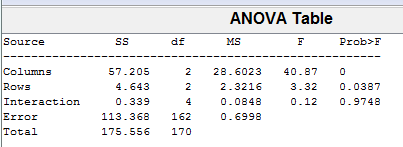
\includegraphics[height=3cm]{fig/anova2_testvalue.png}
		\caption{\textit{{\footnotesize Results for the two-sided ANOVA-test (anova2 in MATLAB) on intellectual engagement after 5, 15 and 30 minutes for each of the three types of controllers (mouse and keyboard, Wii and head mounted display).}}}
		\label{ANOVA_2}
	\end{center}
\end{figure}

The test (fig. \ref{ANOVA_2}) provides an F-statistic of 40.87 regarding the test across the columns (i.e. time). Hence, we can reject the hypothesis of equal mean grades for intellectual engagement after 5, 15 and 30 minutes. The test across the rows (types of controllers) provides an F-statistic of 3.32. In the F-distribution with 2 DF this corresponds with a p-value of 0.0387. With a 5\% level of significance we reject the hypothesis of equal mean for the three types of controllers. The last test has an F-statistic of 0.12 and a corresponding p-value of 0.9748. This provides evidence that there is no interaction between time and controller type in the grades given for intellectual engagement.